%%%%%%%%%%%%%%%%%%%%%%%%%%%%%%%%%%%%%%%%%%%%%%%%%%%%%%%%%%%%%%%%%
% MUW Presentation
% LaTeX Template
% Version 1.0 (27/12/2016)
%
% License:
% CC BY-NC-SA 4.0 (http://creativecommons.org/licenses/by-nc-sa/3.0/)
%
% Created by:
% Nicolas Ballarini, CeMSIIS, Medical University of Vienna
% nicoballarini@gmail.com
% http://statistics.msi.meduniwien.ac.at/
%
% Customized for UAH by:
% David F. Barrero, Departamento de Automática, UAH
%%%%%%%%%%%%%%%%%%%%%%%%%%%%%%%%%%%%%%%%%%%%%%%%%%%%%%%%%%%%%%%%%

\documentclass[10pt,compress]{beamer} % Change 10pt to make fonts of a different size
\mode<presentation>

\usepackage[spanish]{babel}
\usepackage{fontspec}
\usepackage{tikz}
\usepackage{etoolbox}
\usepackage{xcolor}
\usepackage{xstring}
\usepackage{listings}
\usepackage{tikz}
\usetikzlibrary{matrix,chains,positioning,decorations.pathreplacing,arrows,shapes}

\usetheme{UAH}
\usecolortheme{UAH}
\setbeamertemplate{navigation symbols}{} 
\setbeamertemplate{caption}[numbered]

%%%%%%%%%%%%%%%%%%%%%%%%%%%%%%%%%%%%%%%%%%%%%%%%%%%%%%%%%%%%%%%%%
%% Presentation Info
\title[Data structures]{Data structures}
\author{\asignatura\\\carrera}
\institute{}
\date{Departamento de Automática}
%%%%%%%%%%%%%%%%%%%%%%%%%%%%%%%%%%%%%%%%%%%%%%%%%%%%%%%%%%%%%%%%%


%%%%%%%%%%%%%%%%%%%%%%%%%%%%%%%%%%%%%%%%%%%%%%%%%%%%%%%%%%%%%%%%%
%% Descomentar para habilitar barra de navegación superior
\setNavigation
%%%%%%%%%%%%%%%%%%%%%%%%%%%%%%%%%%%%%%%%%%%%%%%%%%%%%%%%%%%%%%%%%

%%%%%%%%%%%%%%%%%%%%%%%%%%%%%%%%%%%%%%%%%%%%%%%%%%%%%%%%%%%%%%%%%
%% Configuración de logotipos en portada
%% Opacidad de los logotipos
\newcommand{\opacidad}{1}
%% Descomentar para habilitar logotipo en pié de página de portada
\renewcommand{\logoUno}{Images/isg.png}
%% Descomentar para habilitar logotipo en pié de página de portada
%\renewcommand{\logoDos}{Images/CCLogo.png}
%% Descomentar para habilitar logotipo en pié de página de portada
%\renewcommand{\logoTres}{Images/ALogo.png}
%% Descomentar para habilitar logotipo en pié de página de portada
%\renewcommand{\logoCuatro}{Images/ELogo.png}
%%%%%%%%%%%%%%%%%%%%%%%%%%%%%%%%%%%%%%%%%%%%%%%%%%%%%%%%%%%%%%%%%

%%%%%%%%%%%%%%%%%%%%%%%%%%%%%%%%%%%%%%%%%%%%%%%%%%%%%%%%%%%%%%%%%
%% FOOTLINE
%% Comment/Uncomment the following blocks to modify the footline
%% content in the body slides. 


%% Option A: Title and institute
\footlineA
%% Option B: Author and institute
%\footlineB
%% Option C: Title, Author and institute
%\footlineC
%%%%%%%%%%%%%%%%%%%%%%%%%%%%%%%%%%%%%%%%%%%%%%%%%%%%%%%%%%%%%%%%%

\begin{document}

%%%%%%%%%%%%%%%%%%%%%%%%%%%%%%%%%%%%%%%%%%%%%%%%%%%%%%%%%%%%%%%%%
% Use this block for a blue title slide with modified footline
{\titlepageBlue
    \begin{frame}
        \titlepage
    \end{frame}
}

\institute{\asignatura}

\begin{frame}[plain]{}
	\begin{block}{Objectives}
		\begin{enumerate}
		\item Understand the need to store information in data structures.
		\item Understand the need to use the type of data structure most appropriate according to data processing to be performed in the script.
		\item Know how to use the different types of existing data structure in Python.
		\end{enumerate}
	\end{block}
\end{frame}

{
\disableNavigation{white}
\begin{frame}[shrink]{Table of Contents}
 \frametitle{Table of Contents}
 \tableofcontents
  % You might wish to add the option [pausesections]
\end{frame}
}

\section{Data structures}
\subsection{Introduction}
\begin{frame}{Data structures}{Introduction}
	Programming is about information representation.
	\begin{itemize}
		\item Simple data are easy to represent: Numbers, characters, strings, etc.
	\end{itemize}
	Reality uses to be more complicated.
	\begin{itemize}
		\item A class represent an object.
		\item How can we store several objects?
		\item How can we represent complex data?
	\end{itemize}
	We need powerful mechanisms to store information: Data structures.
\end{frame}

\subsection{Array}
\begin{frame}[fragile]{Java Collections}{Array}
    \begin{columns}
 	   \column{.50\textwidth}
		\begin{center}
		Vector (1-D array)

		\vspace{-0.2cm}

		\begin{tikzpicture} [nodes in empty cells, 
			nodes={minimum width=0.5cm, minimum height=0.5cm}, 
			row sep=-\pgflinewidth, column sep=-\pgflinewidth]
		border/.style={draw}
		\matrix(vector)[matrix of nodes, 
		row 1/.style={nodes={draw=none, minimum width=0.3cm}},
		nodes={draw}]
{
   	\tiny{0} & \tiny{1} & \tiny{2} & \tiny{3}\\
 	$a_{0}$ & $a_{1}$ & $a_{2}$ & $a_{3}$\\
};
		\end{tikzpicture}

		\bigskip

		Matrix (2-D array)
		\vspace{-0.2cm}

		\begin{tikzpicture} [nodes in empty cells, 
			nodes={minimum width=0.5cm, minimum height=0.5cm}, 
			row sep=-\pgflinewidth, column sep=-\pgflinewidth]
		border/.style={draw}
\matrix (matrix)[matrix of nodes, column 1/.style={nodes={draw=none, minimum width=0.3cm,  minimum height=0.3cm}}, 
		row 1/.style={nodes={draw=none, minimum width=0.3cm}},
		nodes={draw}]
{
   	& \tiny{0} & \tiny{1} & \tiny{2} & \tiny{3}\\
 \tiny{0} & $a_{0,0}$ & $a_{0,1}$ & $a_{0,2}$ & $a_{0,3}$\\
 \tiny{1} & $a_{1,0}$ & $a_{1,1}$ & $a_{1,2}$ & $a_{1,3}$\\
 \tiny{2} & $a_{2,0}$ & $a_{2,1}$ & $a_{2,2}$ & $a_{2,3}$\\
};

		\end{tikzpicture}
		\end{center}

  		\column{.50\textwidth}
		Advantajes:
		\begin{itemize}
			\item Very fast
		\end{itemize}

		Disadvantajes:
		\begin{itemize}
			\item Fixed size
            \item Nor supported in Python \textit{by default}
		\end{itemize}
	\end{columns}
\end{frame}

\subsection{Stack and queue}
\begin{frame}{Data structures}{Data structures (I): Stack and queue}
    \begin{columns}
 	   \column{.15\textwidth}
 	   \column{.30\textwidth}
	   	\centering Stack
 	   \column{.30\textwidth}
	   	\centering Queue
 	   \column{.15\textwidth}
    \end{columns}

	\bigskip

    \begin{columns}
 		\column{.15\textwidth}

 	   \column{.30\textwidth}
		\begin{tikzpicture}[draw, minimum width=1cm, minimum height=0.5cm]
			%\draw[help lines] (-3,-2) grid (3,2);
			\node[draw] (in) at (-1,2) {};
			\node[draw] (out) at (1,2) {};
			\matrix (queue)[matrix of nodes, nodes={draw, nodes={draw}}, nodes in empty cells]
			{
				\\ \\ \\ \\
			}; 
			\draw[-latex] (0.25,1) .. controls (0.25,1.5) and (1,1.5) .. (out.south);
			\draw[-latex] (in.south) .. controls (-1, 1.5) and (-0.25,1.5) .. (-0.25,1); 
		\end{tikzpicture}

 		\column{.30\textwidth}
		\begin{tikzpicture}[draw, minimum width=1cm, minimum height=0.5cm]
			%\draw[help lines] (-3,-2) grid (3,2);
			\node[draw] (in) at (-1,2) {};
			\node[draw] (out) at (1,-2) {};
			\matrix (queue)[matrix of nodes, nodes={draw, nodes={draw}}, nodes in empty cells]
			{
	 				\\ \\ \\ \\
			};
			\draw[-latex] (0.25,-1) .. controls (0.25,-1.25) and (1,-1.25) .. (out.north); 
			\draw[-latex] (in.south) .. controls (-1, 1.5) and (-0.25,1.5) .. (-0.25,1);
		\end{tikzpicture} 

 		\column{.15\textwidth}

	\end{columns}

	Operations:
	\begin{itemize}
		\item \texttt{push(value)} and \texttt{pop(value)}
	\end{itemize}
    Implemented as lists in python
\end{frame}

\subsection{lists and hash tables}
\begin{frame}{Data structures}{Lists and hash tables}
    \begin{columns}
 		\column{.1\textwidth}
 	   	\column{.35\textwidth}
	   	\centering Lists\\ \bigskip

			\begin{tikzpicture}[every node/.style={rectangle split, rectangle split parts=2, rectangle split horizontal,minimum height=14pt}, node distance=1em, start chain,
				 every join/.style={->, shorten <=-4.5pt}]

		  		\node[draw, on chain, join] {   };
		  		\node[draw, on chain, join] {   };
		  		\node[draw, on chain, join] {};

		  	\end{tikzpicture} 


		\begin{flushleft}
		Operations:
		\begin{itemize}
			\item \texttt{insert(pos, value)}
			\item \texttt{get(pos)}
		\end{itemize}
		\end{flushleft}

 		\column{.35\textwidth}
		\centering Hash table\\ (associative array, dictionary)
		\bigskip

		\centering \begin{tabular}{|c|c|}\hline
		\textit{Key 1} & Value 1 \\\hline
		\textit{Key 2} & Value 2 \\\hline
		\textit{Key 3} & Value 3 \\\hline
		\textit{Key 4} & Value 4 \\\hline
		\end{tabular}
		
		\begin{flushleft}
		Operations:
		\begin{itemize}
			\item \texttt{put(key, value)}
			\item \texttt{get(key)}
		\end{itemize}
		\end{flushleft}
 		\column{.10\textwidth}
	\end{columns}
\end{frame}

\subsection{Trees}

\begin{frame}{Data structures}{Trees (I)}
	\begin{center}Trees
	\end{center}

\begin{columns}
 	\column{.50\textwidth}
	   	\begin{center}
		\begin{tikzpicture}[level distance=1.3cm,
			level 1/.style={sibling distance=3cm, level distance=1cm},
	  		level 2/.style={sibling distance=1.5cm, level distance=0.8cm}]
	 	\node {Root}
		    child {node {Child}
	      		child {node {Node}}
		    	child {node {Node}}
			    }
			child {node {Level 2}
			    child {node {Level 3}}
			    child {node {Level 3}}
			    };
		\end{tikzpicture}
		\end{center}

		Operations:
		\begin{itemize} 
			\item \texttt{insert()} and \texttt{remove()} 
			\item \texttt{search()} 
		\end{itemize}

		\column{.50\textwidth}
		\begin{center}

		\begin{tikzpicture}[level distance=1.3cm, 
			level 1/.style={sibling distance=3cm}, 
			level 2/.style={sibling distance=1.5cm, level distance=1cm}, 
			level 3/.style={sibling distance=1cm, level distance=0.8cm}] 
			\node {+}
				child {node {x}
				   	child {node {2}}
				   	child {node {+}
						child {node {8}}
					  	child {node {6}}
					}
			 	}
				child {node {5} 
			};
		\end{tikzpicture}

		\begin{equation*}
			2*(8+6)+5
		\end{equation*}

		\end{center}
		\end{columns}
\end{frame}

\begin{frame}{Data structures}{Trees (II)}
    \begin{columns}
 	   \column{.50\textwidth}
	   	\begin{center}
		\vspace{-0.2cm}
		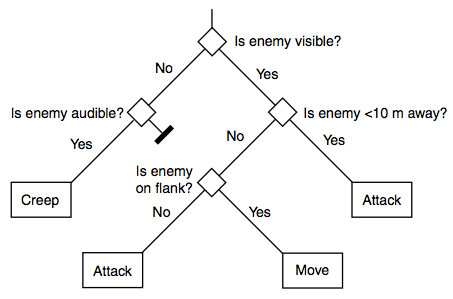
\includegraphics[width=0.9\linewidth]{figs/tree4.png}

		\bigskip

		\vspace{-0.2cm}
		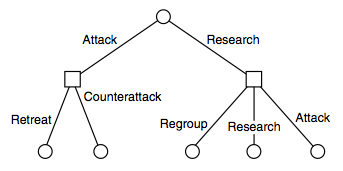
\includegraphics[width=0.9\linewidth]{figs/tree5.png}\\
		\tiny
		Source: Ian Millington, John Funge. ``\textit{Artificial Intelligence for Games}''. Ed. Morgan-Kaufmann. 2009.
		\end{center}

  		\column{.50\textwidth}
	   	\begin{center}
		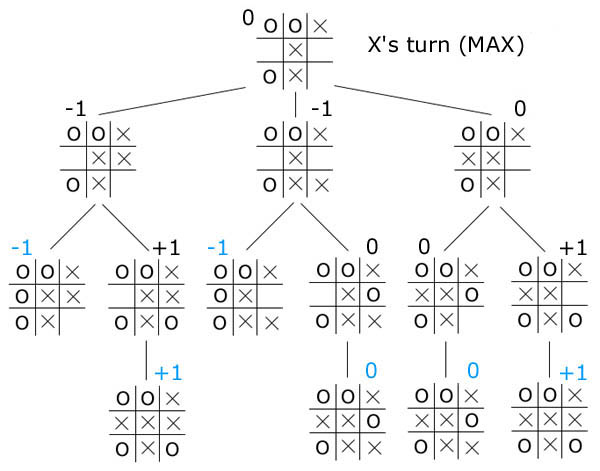
\includegraphics[width=\linewidth]{figs/raya.png}\\
		\tiny{\href{http://www.ocf.berkeley.edu/~yosenl/extras/alphabeta/alphabeta.html}{(Source)}}
	   	\end{center}
		\end{columns}
\end{frame}

\subsection{Graphs}

\begin{frame}{Data structures}{Graphs}
	\begin{center}
	Graphs
	\end{center}

    \begin{columns}
 	   \column{.50\textwidth}
		\vspace{-0.2cm}
		\centering 

		\begin{tikzpicture}[scale=0.4]
    	\tikzstyle{node_style} = [circle,draw=black]
	    \tikzstyle{edge_style} = [draw=black]
		    \node[node_style] (v1) at (-2,2) {2};
		    \node[node_style] (v2) at (2,2) {3};
		    \node[node_style] (v3) at (4,0) {6};
		    \node[node_style] (v4) at (2,-2) {4};
		    \node[node_style] (v5) at (-2,-2) {5};
		    \node[node_style] (v6) at (-4,0) {1};
		    \draw[edge_style]  (v1) edge (v2);
		    \draw[edge_style]  (v2) edge (v3);
		    \draw[edge_style]  (v3) edge (v4);
		    \draw[edge_style]  (v4) edge (v5);
		    \draw[edge_style]  (v5) edge (v6);
		    \draw[edge_style]  (v6) edge (v1);
		    \draw[edge_style]  (v5) edge (v1);
		    \draw[edge_style]  (v5) edge (v2);
		    \draw[edge_style]  (v4) edge (v2);
	    \end{tikzpicture}
		\bigskip

		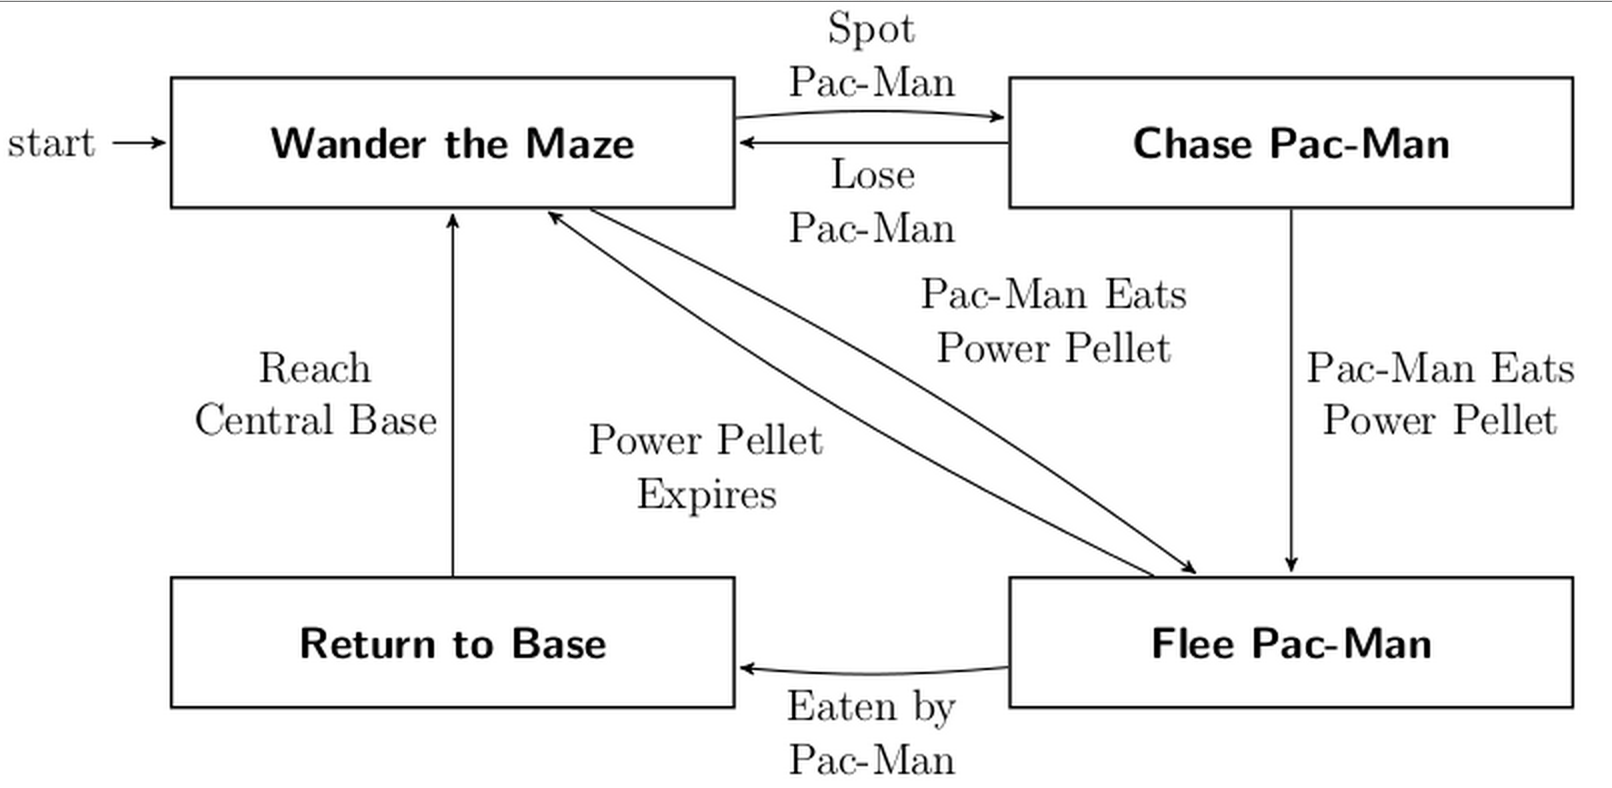
\includegraphics[width=\linewidth]{figs/fsm-pacman.png}\\
		\centering \tiny \href{http://bits.citrusbyte.com/state-design-pattern-with-ruby/}{(Source)}

  		\column{.50\textwidth}

		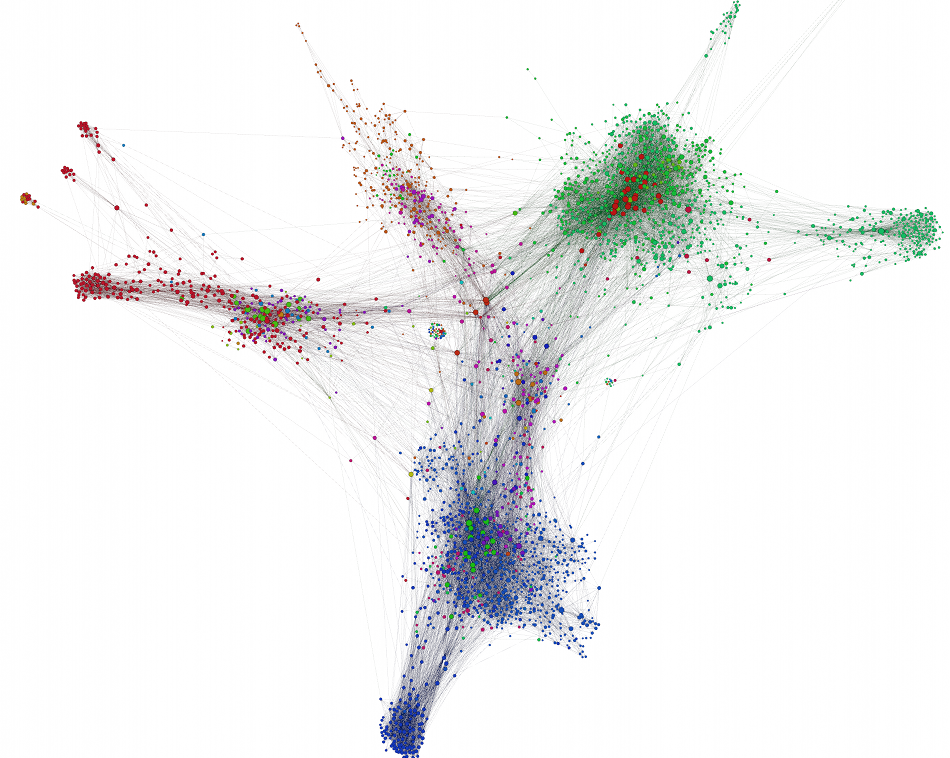
\includegraphics[width=\linewidth]{figs/layout2.png}\\
		\centering \tiny \href{https://gephi.org/features/}{(Source)}


		\normalsize \href{https://www.youtube.com/watch?v=tH9dNESH4ic}{(Video Path-Planning)}

		\end{columns}
\end{frame}

\section{Data structures in Python}
\subsection{Overview}
\begin{frame}{Data structures in Python}{Overview}
	High-level, language-defined data structures:
	\begin{itemize}
		\item Lists.
		\item Tuples and sequences.
		\item Sets.
		\item Dictionaries (associative arrays).
	\end{itemize}
\end{frame}

\subsection{Lists}

\begin{frame}[fragile]{Data structures in Python}{Lists (I)}
    \begin{columns}
 	   \column{.50\textwidth}
	   \begin{block}{List initialization}
	   	\begin{verbatim}
list = [item1, ..., itemN]
\end{verbatim}
	   \end{block}
	   Lists are objects
 	   \column{.50\textwidth}
	Methods:
	\begin{itemize}
		\item \texttt{list.append(x)}
		\item \texttt{list.insert(i, x)}
		\item \texttt{list.remove(x)}
		\item \texttt{list.pop()}
		\item \texttt{list.index(x)}
		\item \texttt{list.count(x)}
		\item \texttt{list.sort()}
		\item \texttt{list.reverse()}
	\end{itemize}
   \end{columns}
\end{frame}

\begin{frame}[fragile]{Data structures in Python}{Lists (II)}
		\begin{exampleblock}{}
		\vspace{-0.4cm}
		\lstinputlisting{code/lists.txt}
		\vspace{-0.2cm}
		\end{exampleblock}
\end{frame}

% uso de len(lista)
% uso de rodajas o slices
\begin{frame}[fragile]{Data structures in Python}{Lists (III)}
    \begin{columns}
 	   \column{.50\textwidth}
		\begin{exampleblock}{Slice notation in lists}
		\vspace{-0.4cm}
		\lstinputlisting{code/list-slices.py}
		\vspace{-0.2cm}
		\end{exampleblock}
   \end{columns}
\end{frame}

% uso de split() y join()
\begin{frame}[fragile]{Data structures in Python}{Lists (IV)}
Sometimes it is useful to \texttt{split} a string to build a list (split) and, conversely, \texttt{join} the elements of a list to build a string
\scriptsize{
		\begin{exampleblock}{join-split.py}
	%	\vspace{-0.4cm}
		\lstinputlisting{code/join-split.py}
%		\vspace{-0.2cm}
		\end{exampleblock}
		}
\end{frame}
% no sé si se han puesto ejemplo de métodos upper(),lower(), find(), strip(), replace(), ...


\subsection{Lists as stacks}
\begin{frame}[fragile]{Data structures in Python}{Lists as stacks}
	Just use two methods: \texttt{append()} and \texttt{pop()}
    
    \begin{columns}
 	   \column{.50\textwidth}
\scriptsize{
		\begin{exampleblock}{}
		\vspace{-0.4cm}
		\lstinputlisting{code/stack.txt}
		\vspace{-0.2cm}
		\end{exampleblock}
		}
    \end{columns}
\end{frame}

\subsection{Lists as queues}
\begin{frame}[fragile]{Data structures in Python}{Lists as queues}
	Queues with lists is not very efficient
	\begin{itemize}
	\item Use instead the \texttt{deque} module from the \texttt{collections} library.
	\end{itemize}
	\normalsize{
		\begin{block}{}
		\vspace{-0.2cm}
		\lstinputlisting{code/deque.txt}
		\vspace{-0.2cm}
		\end{block}
		}
	\normalsize{New Python feature: Modules}
\end{frame}

\subsection{The del statement}
\begin{frame}[plain]{Data structures in Python}{The \texttt{del} statement}
	\texttt{del} is used to delete items and variables

	\footnotesize{
		\begin{block}{}
		\vspace{-0.2cm}
		\lstinputlisting{code/del.txt}
		\vspace{-0.2cm}
		\end{block}
	}

	\normalsize{New Python feature: Error traces}
\end{frame}

\section{Other data structures in Python}
\subsection{Tuples}
\begin{frame}{Other data structures in Python}{Tuples (I)}

	\textbf{Tuple}: A sequence of \textit{ordered} items, very similar to lists.
		\begin{itemize}
		\item \small However they are not the same.
		\item \small Lists are \textit{mutable}, tuples are \textit{inmutable}.
		\item \small Tuples use to contain, \textbf{usually}, heterogeneus items.
		\item \small Lists use to contain, \textbf{usually}, homogeneus items, used to iterate.
        \item Lists and tuples are ordered
		\end{itemize}
	
	    \begin{columns}
 	   \column{.38\textwidth}
 	   \scriptsize{
		\begin{block}{Creation}
		\vspace{-0.2cm}
		\lstinputlisting{code/tuple-declaration.py}
		\vspace{-0.2cm}
		\end{block}
		}
       \vspace{4cm}
 	   \column{.62\textwidth}
 	   \scriptsize{
		\begin{block}{Manipulation}
		\vspace{-0.2cm}
		\lstinputlisting{code/tuple-manipulation.py}
		\vspace{-0.3cm}	
		\end{block}
		}
		\vspace{2.9 cm}

	\end{columns}
\end{frame}

\begin{frame}{Other data structures in Python}{Tuples (II)}
 	  \vspace{-0.2cm}
 	   \tiny{
		\begin{block}{\scriptsize{Modification}}
		
		\vspace{-0.2cm}
		\lstinputlisting{code/tuple-manipulation1.py}
		\vspace{-0.2cm}
		
		\end{block}
   }
\end{frame}

\subsection{Sets}
\begin{frame}{Other data structures in Python}{Sets (I)}
\vspace{-0.2cm}
	\textbf{Set}: A collection of items, unordered with no duplicates.
		\begin{itemize}
		\item \small{Membership testing.}
		\item \small{Eliminating duplicate entries.}
		\item \small{Math operations: \texttt{union()}, \texttt{intersection()} and \texttt{difference()}.}
		\end{itemize}
\vspace{-0.2cm}
    \begin{columns}
 	   \column{.45\textwidth}
 	   \scriptsize{
		\begin{block}{Creation (I)}
		\vspace{-0.2cm}
		
		\lstinputlisting{code/set-declaration.py}
		\vspace{-0.2cm}
		\end{block}
		}
		

 	   \column{.55\textwidth}
 	  \scriptsize{
 	   \begin{block}{Creation (II)}
		\vspace{-0.2cm}
		
		\lstinputlisting{code/set-manipulation1.py}
		\vspace{-0.2cm}
		
		\end{block}
		\vspace{0.3cm}
		}
	\end{columns}
\end{frame}

%\begin{frame}{Other data structures in Python}{Sets (II)}
	

 	   %\scriptsize{
% 	   \begin{block}{Manipulation (I)}
%		\vspace{-0.2cm}
%		\lstinputlisting{code/set-manipulation.py}
%		\vspace{-0.2cm}
%		\end{block}		
	%	}
%\end{frame}		

\begin{frame}{Other data structures in Python}{Sets (II). Modification}
 	  
 	   \tiny{
		\begin{block}{}
		
		\vspace{-0.2cm}
		\lstinputlisting{code/set-manipulation2.py}
		\vspace{-0.2cm}
		
		\end{block}
   }
\end{frame}

\begin{frame}[plain]{Other data structures in Python}{Sets (III). Modification}
 	\vspace{-0.24cm}  
 	   \tiny{
		\begin{block}{}
		
		\vspace{-0.2cm}
		\lstinputlisting{code/set-manipulation3.py}
		\vspace{-0.2cm}
		
		\end{block}
   }

	\vspace{0.1cm}
    \normalsize \textbf{Sequence}: All types that behaves like sequences: Strings, lists and tuples.
\end{frame}

\subsection{Dictionaries}
\begin{frame}{Other data structures in Python}{Dictionaries (I)}
	\textbf{Dictionary}: A collection of pairs \texttt{<key, value>}
		\begin{itemize}
		\item Also named as \textit{associative array}, very similar to hash maps.
		\item Lists are indexed with a number, dictionaries use keys.
		\item Key: Numbers, strings, tuples and any inmutable type.
		\end{itemize}

		\vspace{-0.3cm}
    \begin{columns}
 	   \column{.50\textwidth}
		\begin{block}{Creation}
		\vspace{-0.2cm}
		\lstinputlisting{code/dict-declaration.py}
		\vspace{-0.2cm}
		\end{block}
		\vspace{0.7cm}

 	   \column{.50\textwidth}
		\begin{block}{Manipulation}
		\vspace{-0.2cm}
		\lstinputlisting{code/dict-manipulation.py}
		\vspace{-0.2cm}
		\end{block}

	\end{columns}
\end{frame}
% alguna cuestión más sobre su manipulación. Por ejemplo, se pueden borrar todos sus elementos con clear()
% len(dicc), dicc.has_key(k) o k in dicc, dicc.keys() como aparece en el ejemplo anterior: lista de claves, dicc.items() -los elementos como lista de pares

\begin{frame}{Other data structures in Python}{Dictionaries (II)}
	Dictionaries can be iterated by key or by value
		\begin{itemize}
		\item Loop syntax is slightly different
		\item \texttt{item()} method
		\end{itemize}

    \begin{columns}
 	   \column{1.1\textwidth}
		\begin{block}{Dictionary iteration}
		\vspace{-0.2cm}
		\lstinputlisting{code/dict-iteration.py}
		\vspace{-0.2cm}
		\end{block}
	\end{columns}
\end{frame}

\subsection{Looping techniques}
\begin{frame}{Other data structures in Python}{Looping techniques (I)}
	A bunch of useful functions for looping
		\begin{description}
		\item[\texttt{enumerate()}] Retrieve position index and value.
		\item[\texttt{zip()}] Pair two or more sequences.
		\item[\texttt{sorted()}] Iterate in order.
		\item[\texttt{reversed()}] Iterate in reverse order.
		\end{description}
\end{frame}

\begin{frame}{Other data structures in Python}{Looping techniques (II)}
    \begin{columns}
 	   \column{\textwidth}
		\begin{block}{enumerate()}
		\vspace{-0.2cm}
		\lstinputlisting{code/enumerate.py}
		\vspace{-0.2cm}
		\end{block}

		\begin{block}{zip()}
		\vspace{-0.2cm}
		\lstinputlisting{code/zip.py}
		\vspace{-0.2cm}
		\end{block}

	\end{columns}
\end{frame}

\begin{frame}{Other data structures in Python}{Looping techniques (III)}
    \begin{columns}
 	   \column{\textwidth}
		\begin{block}{sorted()}
		\vspace{-0.2cm}
		\lstinputlisting{code/sorted.py}
		\vspace{-0.2cm}
		\end{block}

		\begin{block}{reversed()}
		\vspace{-0.2cm}
		\lstinputlisting{code/reversed.py}
		\vspace{-0.2cm}
		\end{block}

	\end{columns}
\end{frame}

\subsection{More on conditions}
\begin{frame}{Other data structures in Python}{More on conditions (I)}
    %\vspace{-0.2cm}
    \begin{columns}
    \column{.35\textwidth}
		\centering \textit{Comparison operators}
		\centering \begin{tabular}{cl}
		== & Equal to 	 \\
		!= & Not equal to \\
		<> & Similar to != \\
           & (deprecated in 3.x)\\
		>  &Greater than \\
		<  &Less than \\
		>= &Less or eq. to\\
		<= &Less or eq. to\\
		\end{tabular}
		
		\bigskip
		\centering \textit{Conditional operators}
		\centering \begin{tabular}{cl}
		\texttt{and} &AND\\
		\texttt{or}	 &OR \\
		\texttt{not} &Negation \\
		\end{tabular}

    \column{.65\textwidth}
		\begin{itemize}
		\item Widely used in loops and conditions
		\item Result: \texttt{true} or \texttt{false} 
			\begin{itemize}
			\item Python supports boolean variables
			\item The result is a boolean
			\end{itemize}
		\item Truth tables represent the conditional operators
		\end{itemize}

        \bigskip

		\centering \textit{Truth tables}
		\smallskip
    	\begin{columns}
    	\column{.1\textwidth}
    	\column{.4\textwidth}
		\footnotesize{
		\centering \begin{tabular}{|c|c|}\hline
		A	   &TTFF \\
		B 	   &TFTF \\\hline
		A and B &TFFF \\\hline
		\end{tabular}
		}
    	\column{.4\textwidth}
		\footnotesize{
		\centering \begin{tabular}{|c|c|}\hline
		A	 &TTFF \\
		B 	 &TFTF \\\hline
		A or B &TTTF \\\hline
		\end{tabular}
		}
    	\column{.1\textwidth}
		\end{columns}
	\end{columns}
\end{frame}

\begin{frame}{Other data structures in Python}{More on conditions (II)}
	\begin{exampleblock}{Example}
		\vspace{-0.2cm}
		\lstinputlisting[language=python, basicstyle=\ttfamily\scriptsize]{code/ComparisonDemo.py}
		\vspace{-0.2cm}
	\end{exampleblock}
\end{frame}

\begin{frame}{Other data structures in Python}{More on conditions (III)}
    %\vspace{-0.2cm}
    \begin{columns}
    \column{.35\textwidth}
		\centering \textit{Identity operators}
		\centering \begin{tabular}{cl}
		\texttt{is} 	& Same objects 	 \\
		\texttt{is not} & Not same objects \\
		\end{tabular}
		
		\bigskip
		\centering \textit{Membership operators}
		\centering \begin{tabular}{cl}
		\texttt{in} 	& Contained    \\
		\texttt{not in}	& Not contained\\
		\end{tabular}

    \column{.65\textwidth}
		\begin{itemize}
		\item Identity operators compare \texttt{objects}
			\begin{itemize}
			\item We will study objects later, do not worry right now
			\end{itemize}
		\item Membership valid on sequences
			\begin{itemize}
			\item Remember: A sequence is a string, tuple or list
			\end{itemize}
		\end{itemize}
	\end{columns}
	\begin{block}{Example}
		\vspace{-0.2cm}
		\lstinputlisting[language=python, basicstyle=\ttfamily\scriptsize]{code/ComparisonDemo2.py}
		\vspace{-0.2cm}
	\end{block}
\end{frame}



\section{Summary}
\begin{frame}{Summary}
	
\centering \begin{tabular}{l|c|c|l}
\hline
\sc    & \sc{Mutable} & \sc{Ordered} & \sc Initialization  \\\hline
List   & Yes & Yes & \texttt{li = [1, 2, 3]} \\
Tuple  & No  & Yes & \texttt{tu = (1, 2, 3)} \\
	   & & & \texttt{tu = 1, 2, 3} \\
Set    & No & No & \texttt{se = \{1, 2, 3\}} \\
Dictionary& Yes & No & \texttt{dic = \{'abc' : 1, 'bca' : 2\}} \\\hline
\end{tabular}
\end{frame}

\end{document}

% inmersión en python
\appendix
\section<Bibliographic references>*{\appendixname}
\subsection<Bibliographic references>*{Bibliographic references}

\begin{frame}[plain,allowframebreaks]
  \frametitle<presentation>{Bibliographic references}

  \begin{thebibliography}{4}

  \beamertemplatebookbibitems
  % libro
   \bibitem{vanRosum}[van Rosum, 2012]
    G. van Rossum, Jr. Fred L. Drake.
    \newblock \emph{Python Tutorial Release 3.2.3, chapter 5}.
    \newblock Python Software Foundation, 2012. 
  % libro
   \bibitem{Marzal}[Marzal, 2014]
     A. Marzal Varó, I. Gracia Luengo, P. García Sevilla.
    \newblock \emph{Introducción a la programación con Python 3, capítulo 5}.
    \newblock Universidad Jaime I.
    
     \bibitem{Bahit}[Bahit, 2008]
     E. Bahit.
    \newblock \emph{Curso: Python para principiantes}.
    \newblock Creative Commons Atribución-NoComercial 3.0, 2012.
    
  % libro
   

  \bibitem{Pilgrim}[Pilgrim, 2004]
  M. Pilgrim.
    \newblock \emph{Dive into Python}.
    \newblock Ed. Prentice Hall, 2004.
   
    
 
  \end{thebibliography}
\end{frame}




\end{document}
